\newpage
\usecasebase{Visualizzazione menù}
\label{usecase:Visualizzazione menù}

\begin{figure}[h]
	\centering
	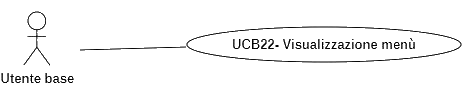
\includegraphics[width=0.7\textwidth]{./uml/UCB22.png} 
	\caption{Visualizzazione menù}
	\label{fig:UCB22}
  \end{figure}


\begin{itemize}
	\item \textbf{Attore principale:} Utente base.

	\item \textbf{Precondizioni:}
	      \begin{itemize}
		      \item L'Utente ha eseguito correttamente l'accesso al Sistema come
		            Utente base (vedi \autoref{usecase:Effettua accesso}).
	      \end{itemize}

	\item \textbf{Postcondizione:} L'Utente base visualizza tutte le pietanze presenti nel menù di un determinato ristorante.

	\item \textbf{Scenario principale:}
	      \begin{enumerate}
		      \item L'Utente base visualizza tutti i piatti e le pietanze presenti nel menù di un ristorante;
		      \item Il Sistema presenta all'Utente base il menù del ristorante con le seguenti informazioni per ogni pietanza:
		            \begin{itemize}
			            \item Nome.
			            \item Immagine della pietanza.
			            \item Ingredienti.
			            \item Prezzo.
			            \item Dettagli sulle allergie e intolleranze.
		            \end{itemize}
	      \end{enumerate}
\end{itemize}
